\subsection{Light Collection for Proportional Scintillation Signal (S2)}
\label{secLCEs2}

A proper simulation of the proportional scintillation signal (S2) is an essential requirement for the correct reconstruction of the event vertex (see Chapter~\ref{chPositionReconstruction}). The simulated PMT response is used to `train' all three reconstruction algorithms developed for the XENON100 experiment.

The stack of the top electrode meshes is shown in Fig.~\ref{figAnodeStack}. The copper `screen' on  the top of the PTFE holders supporting the top electrodes (Fig.~\ref{figAnodeStack_2}) prevents the collection of the S1 signal from the charge insensitive region at the edge of the TPC.

\begin{figure}[!h]
\centering
\subfigure[]{
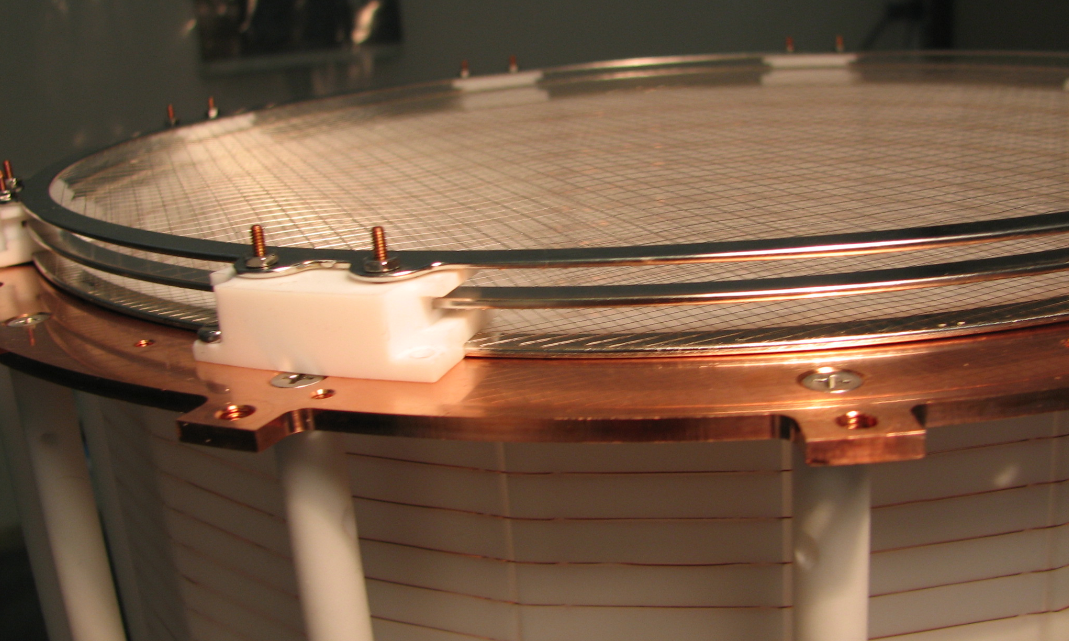
\includegraphics[height=0.3\linewidth]{plots/LCEs2/AnodeStack.png}
\label{figAnodeStack_1}}
\subfigure[]{
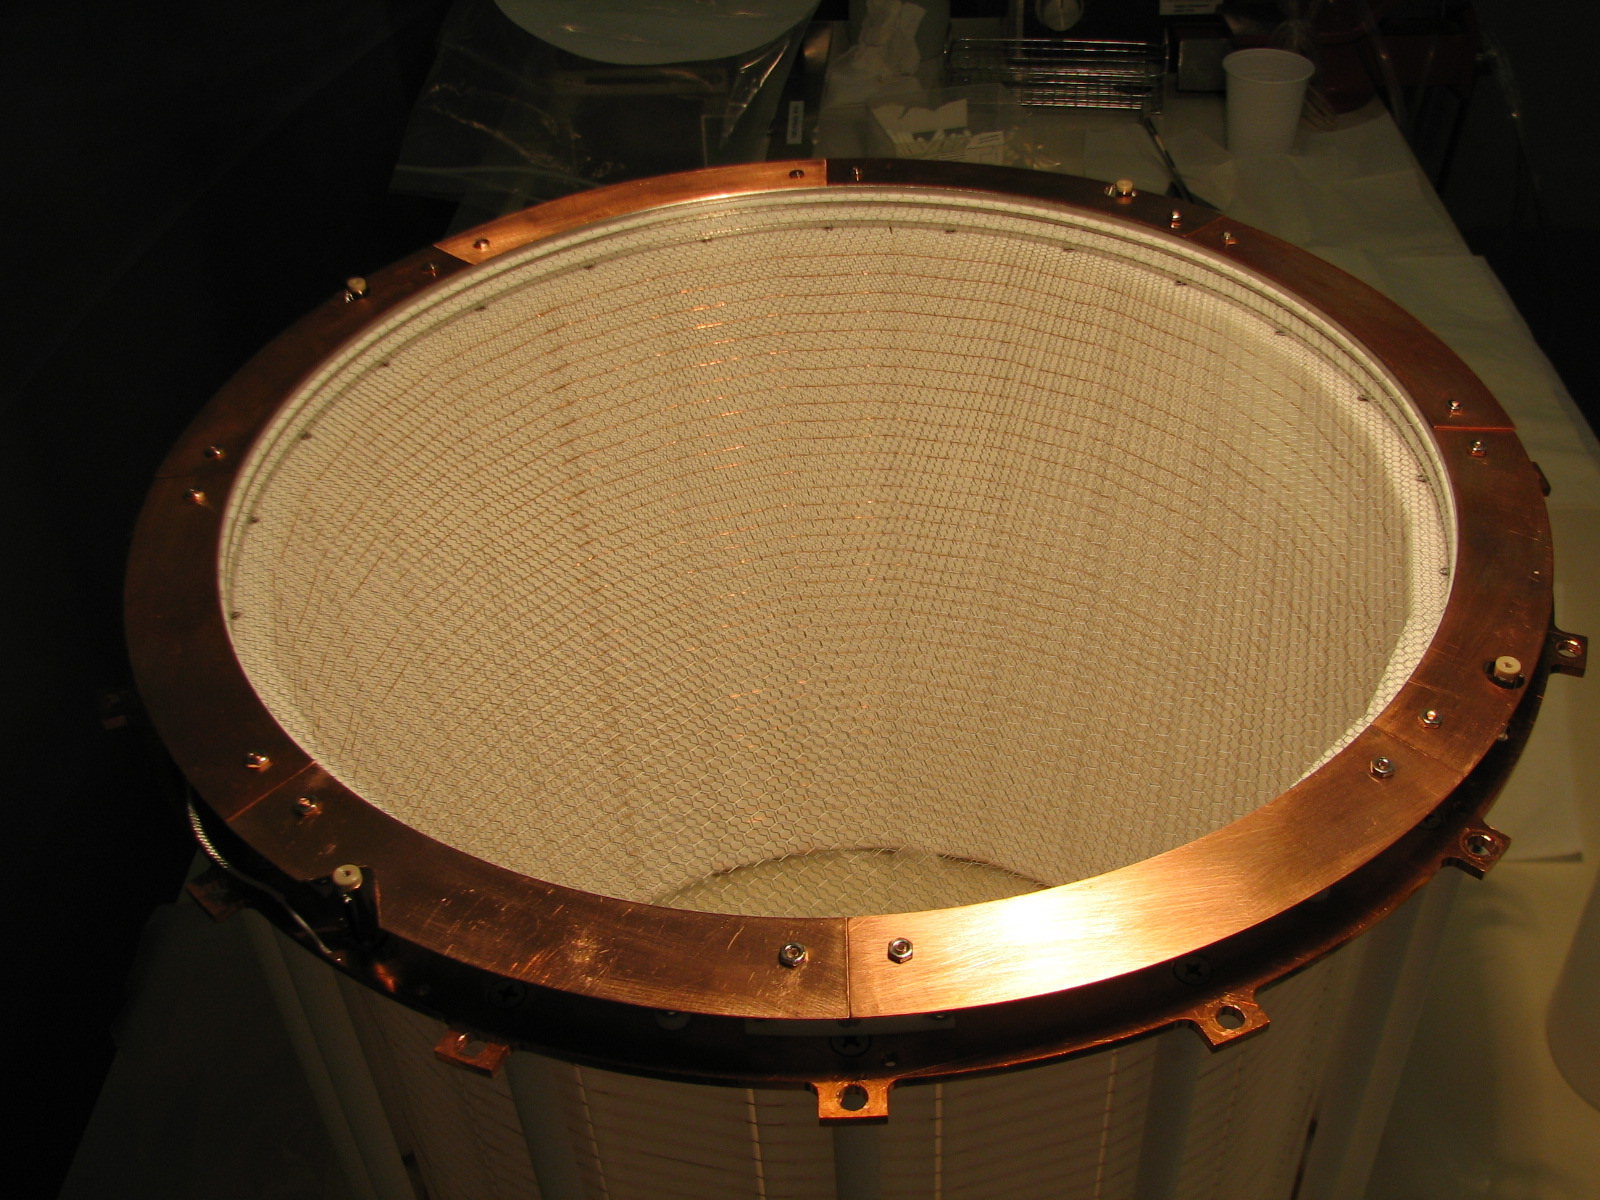
\includegraphics[height=0.3\linewidth]{plots/LCEs2/CopperScreenPhoto.png}
\label{figAnodeStack_2}}
\caption[Top electrode meshes]{A stack of the three top electrode meshes (a). On the top it is covered with a copper screen, in order to prevent the charge collection in the S1 insensitive region above stainless steel the support rings.}
\label{figAnodeStack}
\end{figure}

A screenshot of the Monte Carlo simulation of S2 light propagation with GEANT4 is shown in Fig.~\ref{figMCs2_1}. The light source is modeled in a similar way as described in Section~\ref{secLCEs1}: mono-energetic UV optical photons with an energy of 7~eV are isotropically generated within a thin disk in the gas phase, (3.75$\pm$0.50)~mm above the liquid-gas interface, where electro-luminescence process takes place. 

\begin{figure}[!b]
\centering
\subfigure[]{
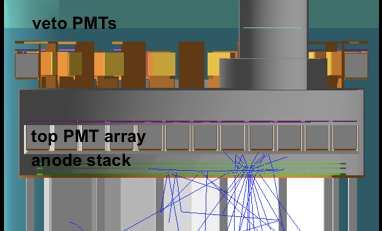
\includegraphics[width=0.475\linewidth]{plots/LCEs2/G4_S2simulation.png}
\label{figMCs2_1}}
\subfigure[]{
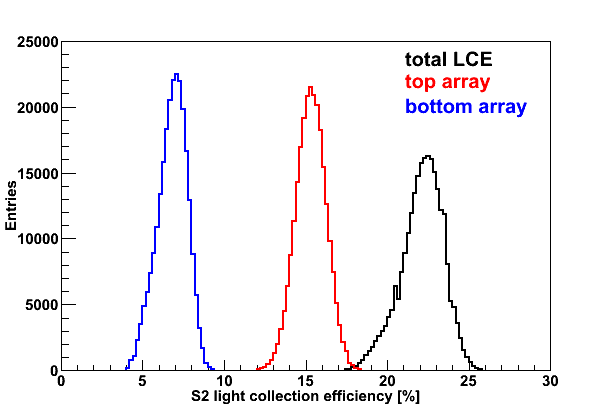
\includegraphics[width=0.475\linewidth]{plots/LCEs2/LCE_S2_comparison.png}
\label{figMCs2_2}}
\caption[Monte Carlo simulation of the proportional scintillation signal (S2)]{Monte Carlo simulation of the proportional scintillation signal (S2): (a) - GEANT4 model. Blue lines show the photon tracks. (b) - simulated light collection efficiency.}
\label{figMCs2}
\end{figure}

The optical boundary between the xenon in the gas phase and the copper screen has been defined using a  `dielectric-metal' interface, which includes absorption and reflection as boundary processes. As a surface model for the copper, the `G4LogicalSkinSurface' has been chosen, applicable when a logical volume is entirely surrounded by a given surface, and the `GLISUR' model has been used~\cite{LogicalSkinSurface}. Copper surface finish has been defined as `ground', which corresponds to a rough surface.

The S2 LCE is shown in Fig.~\ref{figMCs2_2}. The total LCE is 23\% in average, and the ratio of the signal detected on the top and bottom PMT arrays is $\sim$2.3. These values do not include the QE and CE of the PMTs, Frenel losses, and transmission efficiency of the synthetic silica windows.

%   With a copper screen, a slight increase of the light collection by the top PMT array has been observed (by a factor of 1.2$\sim$). Simultaneously, light collection by the bottom PMT array decreased almost twice. As a result, the total LCE (amount of light detected by all 178 PMTs in the target volume) decreased from 26\% to 22\%.
\begin{figure}[!t]
\centering
\subfigure[]{
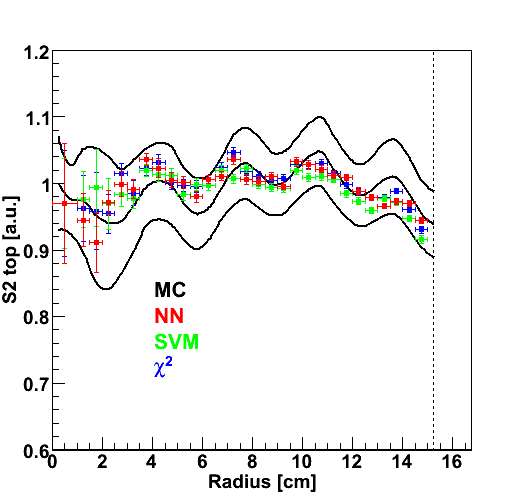
\includegraphics[width=0.475\linewidth]{plots/LCEs2/40keV_S2topvsR_MC1andData.png}
\label{figLCEs2_1}}
\subfigure[]{
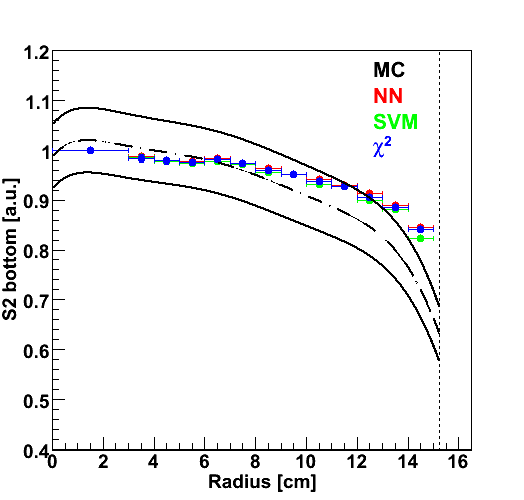
\includegraphics[width=0.475\linewidth]{plots/LCEs2/40keV_S2botvsR_MC1andData.png}
\label{figLCEs2_2}}
\caption[Relative collection efficiency for S2 signal in the measured data and Monte Carlo simulations]{Relative collection efficiency for S2 signal in the measured data and Monte Carlo simulations, for the top (a) and bottom (b) PMT arrays. Horizontal ticks on the graph show the width of the slice, and vertical errors bars present the error of the mean value extracted from a Gaussian fit. The Monte Carlo data is shown together with $\pm\sigma$ band.}
\label{figLCEs2}
\end{figure}

\begin{figure}[!b]
\centering
\subfigure[top]{
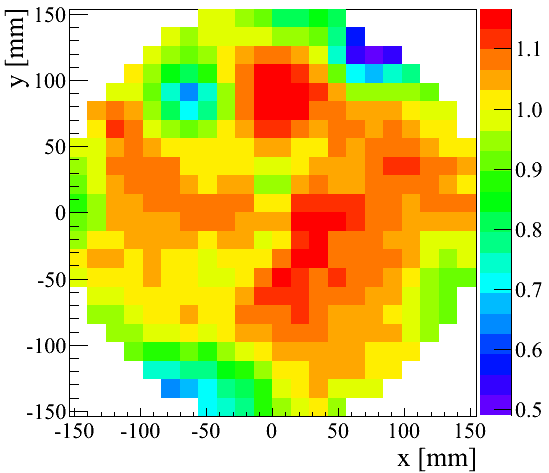
\includegraphics[width=0.475\linewidth]{plots/LCEs2/S2topCorrectionMap.png}
\label{figCorrectionMapS2_1}}
\subfigure[bottom]{
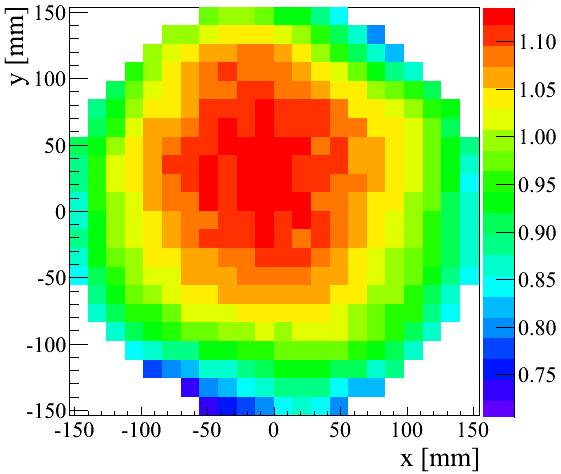
\includegraphics[width=0.475\linewidth]{plots/LCEs2/S2bottomCorrectionMap.png}
\label{figCorrectionMapS2_2}}
\caption[Spatial correction maps for S2 detected by the top and bottom PMT arrays]{Spatial correction maps for S2 detected by the top (a) and bottom (b) PMT arrays, measured with a $^{137}$Cs calibration with a lowered anode voltage (2.2~kV). Figures published in Ref.~\cite{xe100-instrument}. }
\label{figCorrectionMapS2}
\end{figure}

The results of the simulation have been compared to the measured data. Since the amount of light produced  by proportional scintillation is large (typically $\sim$2 orders of magnitude higher than corresponding S1), this can result in non-linear effects in the PMTs (see Section~\ref{secPosRecSaturation}). Hence, a $^{137}$Cs calibration has not be used for this study. The relative LCE for the measurements has thus been calculated for the 40~keV peak, produced by inelastic neutron interactions with $^{129}$Xe atoms during calibration with an $^{241}$Am-Be source. The detector is divided into 15 rings with a width of 1~cm each, and the response to the 40~keV is calculated by fitting a Gaussian to the observed distributions. The results of the study are presented in Fig.~\ref{figLCEs2_1} for the top PMT array, and in Fig.~\ref{figLCEs2_2} for the bottom PMTs. The graphs are normalized to the LCE value computed in the first bin, within 1~cm in the center of the target volume, where the maximum LCE is expected.

The Monte Carlo model and the measured LCE for the S2 light are in a good agreement for the top PMT array, which is of high importance for the correct reconstruction of the event vertex. For the bottom array, the simulated LCE does not correctly reproduce the measured distribution. This is suspected to be due to non-homogeneity of the PTFE walls of the TPC, which supports the field shaping rings made out of copper wires, with much lower reflectivity to UV light than PTFE.

In the analysis of XENON100 data, the signals on both arrays are corrected independently. The Monte Carlo results have not been used for this purpose. Instead, the spatial correction maps have been determined in the same way as for the S1 LCE, using 40~keV and~164 keV gamma lines from inelastic neutron scattering and neutron activation, respectively, and $^{137}$Cs calibration data acquired with lowered anode voltage. The correction maps for S2 detected by the top and bottom arrays are shown in Fig.~\ref{figCorrectionMapS2_1} and Fig.~\ref{figCorrectionMapS2_2}, respectively. 
The results obtained with these lines agree within the uncertainties of the measurements.

The spatial anisotropy observed on the top array is due to a slight warping of the mesh along the stretching directions, and due to regions of reduced S2 sensitivity where individual PMTs do not function (see Fig.~\ref{figPMTarrangement}). For the bottom array, the impact of non function PMTs and mesh warping is irrelevant, since the S2 light is spread over the full array. Within the radius of 13.5~cm, the maximum correction is about 20\% with a RMS of 6.6\%. The corrections are locally larger on the top array, but the RMS value (8.7\%) is only slightly higher than on the bottom array. 

